\documentclass[10pt,a4paper,twocolumn]{article}
\usepackage[utf8]{inputenc}
\usepackage[T1]{fontenc}
\usepackage[spanish,es-tabla,es-nodecimaldot,es-noshorthands]{babel}
\usepackage{lmodern}
\usepackage{microtype}
\usepackage[margin=1.7cm,columnsep=0.6cm]{geometry}
\usepackage{amsmath,amssymb}
\usepackage{graphicx}
\usepackage{booktabs}
\usepackage{caption}
\usepackage{enumitem}
\usepackage{cite}
\usepackage[hidelinks]{hyperref}

\graphicspath{{figures/}}
\captionsetup{font=small,labelfont=bf}
\setlist{itemsep=0.1em,topsep=0.25em,leftmargin=1.2em}
\setlength{\emergencystretch}{2em}
\newcommand{\archivo}[1]{\texttt{\small #1}}

\title{\textbf{Fresh: probador virtual de barbería\\con computación gráfica}\\[0.3em]
\normalsize Resumen ejecutivo del proyecto final de CS4016}
\author{Kalos Lazo Mera \qquad Sofía Herrera \qquad Gianpier Segovia\\
\small Universidad de Ingeniería y Tecnología (UTEC), Lima, Perú}
\date{Noviembre de 2026}

\begin{document}

\twocolumn[{%
  \csname @twocolumnfalse\endcsname
  \maketitle
  \begin{abstract}
  \noindent Fresh es una aplicación web para probarse barbas, tintes y cortes de pelo sobre la propia foto o con la cámara, antes de ir a la barbería. En lugar de generar una cara nueva con un modelo generativo, mide la geometría de la cara y del pelo de la persona y compone cada estilo sobre la foto original. Los modelos preentrenados solo ubican la cara, el pelo y la mano; todo lo demás es implementación propia: una triangulación de Delaunay con el algoritmo de Fortune, un \emph{warp} afín por triángulo, un tinte en CIELAB, un motor de ocho cortes con relleno \emph{pull-push}, física de la barba con Verlet, gaussianas 2D ajustadas con gradientes analíticos y un visor de \emph{Gaussian Splatting} 3D en WebGL2. El sistema corre en CPU, procesa una foto en 0,1 a 2,5~s y se reproduce con un solo comando de Docker.

  \medskip
  \noindent\textbf{Palabras clave:} triangulación de Delaunay, \emph{warp} afín, CIELAB, \emph{inpainting}, Verlet, \emph{Gaussian Splatting}.
  \end{abstract}
  \bigskip
}]

\section{Introducción}

Cortarse el pelo, dejarse la barba o teñirse son decisiones que se toman a ciegas: el resultado se ve cuando ya está hecho. Las aplicaciones que existen pegan una imagen encima de la foto, sin seguir la forma de la cara ni la luz, o usan modelos generativos que inventan la cara completa, pierden la identidad y necesitan GPU.

Fresh aborda el problema con computación gráfica: modela la cara y el pelo de la persona y compone sobre la foto original las capas necesarias (barba, color, pelo corto y piel). Así el resultado conserva la identidad, la iluminación y la textura. Las contribuciones son:
\begin{itemize}
  \item un pipeline en el que los modelos solo ubican y el código del equipo hace toda la geometría y el render (unas 4\,000 líneas propias frente a 600 que llaman a modelos);
  \item un motor de cortes que quita el pelo, reconstruye el fondo y hace crecer pelo corto con la luz de la foto;
  \item un tinte en CIELAB que conserva los mechones y puede teñir también la barba;
  \item física de la barba y un juego de afeitado en vivo;
  \item gaussianas 2D y 3D implementadas desde cero, con un visor propio en WebGL2.
\end{itemize}

\begin{figure*}[t]
  \centering
  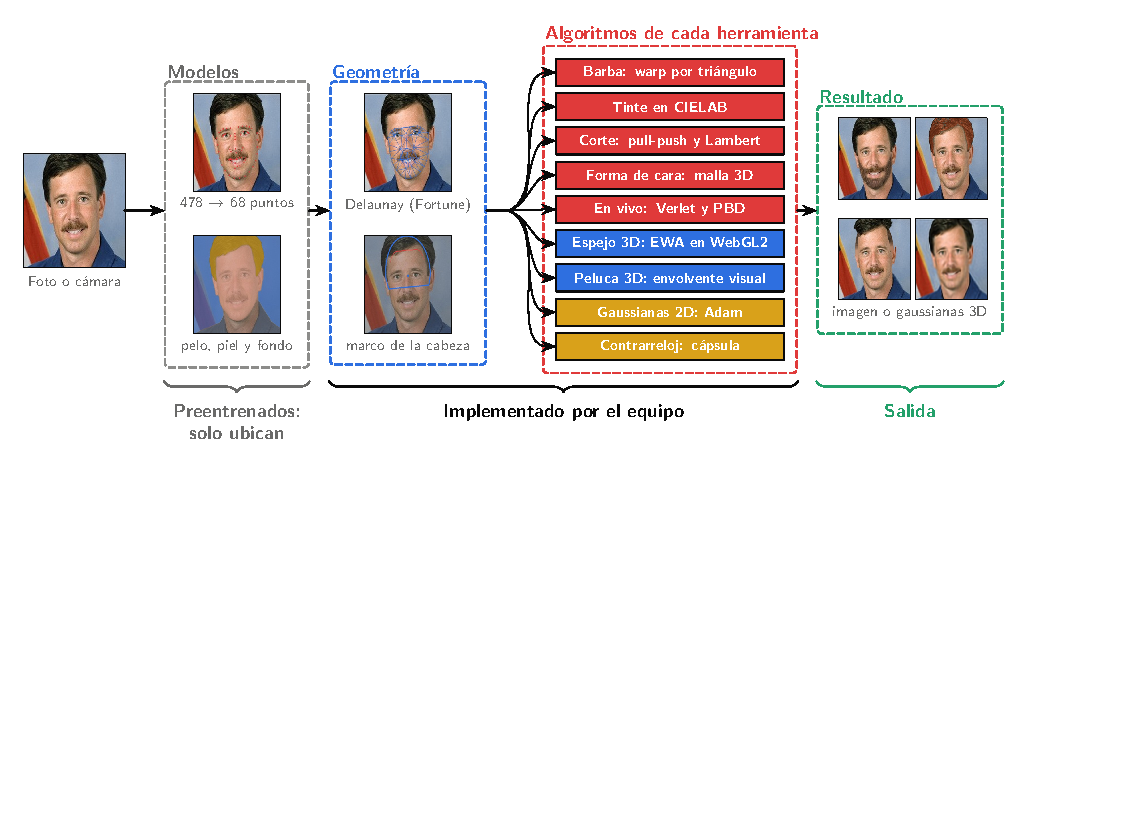
\includegraphics[width=0.92\textwidth]{diagrama_general.pdf}
  \caption{Pipeline de Fresh. En gris, los modelos preentrenados, que solo ubican; el resto lo implementó el equipo. Los colores de las herramientas siguen los grupos de la interfaz: Estilos (rojo), 3D (azul) y Juegos (amarillo).}
  \label{fig:general}
\end{figure*}

\section{Visión general}

La figura~\ref{fig:general} muestra el recorrido de una foto. MediaPipe~\cite{kartynnik2019,lugaresi2019} entrega 478 puntos de la cara, que se convierten a los 68 puntos estándar, y un segmentador marca pelo, piel y fondo. Para el tinte se puede usar en su lugar un YOLOv8n-seg~\cite{jocher2023} que el equipo ajustó con Figaro1k~\cite{svanera2016} y CelebAMask-HQ~\cite{lee2020} (mAP50 de máscara de 0,968).

Con los puntos se arma una malla de Delaunay y un \emph{marco de la cabeza}: coordenadas $(x,y)$ medidas en anchos de cabeza, con origen entre las orejas. Así un mismo parámetro vale para una foto de 600~px y para una de 4000~px. Sobre esa geometría, cada herramienta aplica su algoritmo y devuelve una imagen compuesta o, en el 3D, gaussianas que dibuja el navegador.

El servidor es un único proceso de FastAPI dentro de un contenedor Docker. El modo en vivo y el juego guardan estado entre cuadros, y cada llamada al pipeline corre en un hilo detrás de un candado. La interfaz es HTML y JavaScript sin compilación.

\section{Métodos}

\subsection{Malla de Delaunay con Fortune}

La triangulación de Delaunay~\cite{delaunay1934} evita triángulos finos, que estirarían la textura. Se construye con el barrido de Fortune~\cite{fortune1987}: cada evento de círculo es un vértice de Voronoi y aporta un triángulo cuyo círculo circunscrito está vacío. Nuestra \emph{beach line} es una lista enlazada, así que la implementación es $O(n^2)$ en el peor caso, en vez del $O(n\log n)$ que se logra con un árbol; con 83 puntos tarda 3~ms. Contra Bowyer--Watson~\cite{bowyer1981,watson1981}, Fortune encuentra además un triángulo válido del borde de la mandíbula que el otro método pierde por su supertriángulo finito. Para los casos degenerados (puntos cocirculares, como en una grilla) se perturban los puntos en una millonésima del tamaño de la nube y se descartan los triángulos sin área.

\subsection{Barba}

Una barba real de CelebAMask-HQ se deforma a la cara con un \emph{warp} afín por triángulo: para cada píxel del triángulo destino se resuelve la afín inversa, se prueba si está dentro con coordenadas baricéntricas y se lee el origen con interpolación bilineal propia. La barba se compone en tres capas: \emph{multiply}, $C=(1-\alpha)\,b+\alpha\,b\,m$, que oscurece sin tapar la luz de la piel; hebras con curvas de Bézier; y la alta frecuencia de la plantilla, que aporta los pelos reales sin su brillo.

\subsection{Tinte en CIELAB}

En CIELAB~\cite{cie2004} la luminosidad está separada del color. La luminosidad del pelo se divide en sombreado $s=G_\sigma(L)-\bar L$ y detalle $d=L-G_\sigma(L)$, y la nueva luminosidad es
\begin{equation}
  L'=0{,}72\,L_t+0{,}28\,\bar L+k\,(0{,}8\,s+1{,}2\,d),
\end{equation}
con $k=\mathrm{clip}(20/s_L,\,0{,}9,\,1{,}8)$ para normalizar el contraste. La base va hacia el tinte y el detalle se conserva, así un pelo negro puede quedar rubio. El croma baja en las sombras, como en un pigmento real.

\begin{figure*}[t]
  \centering
  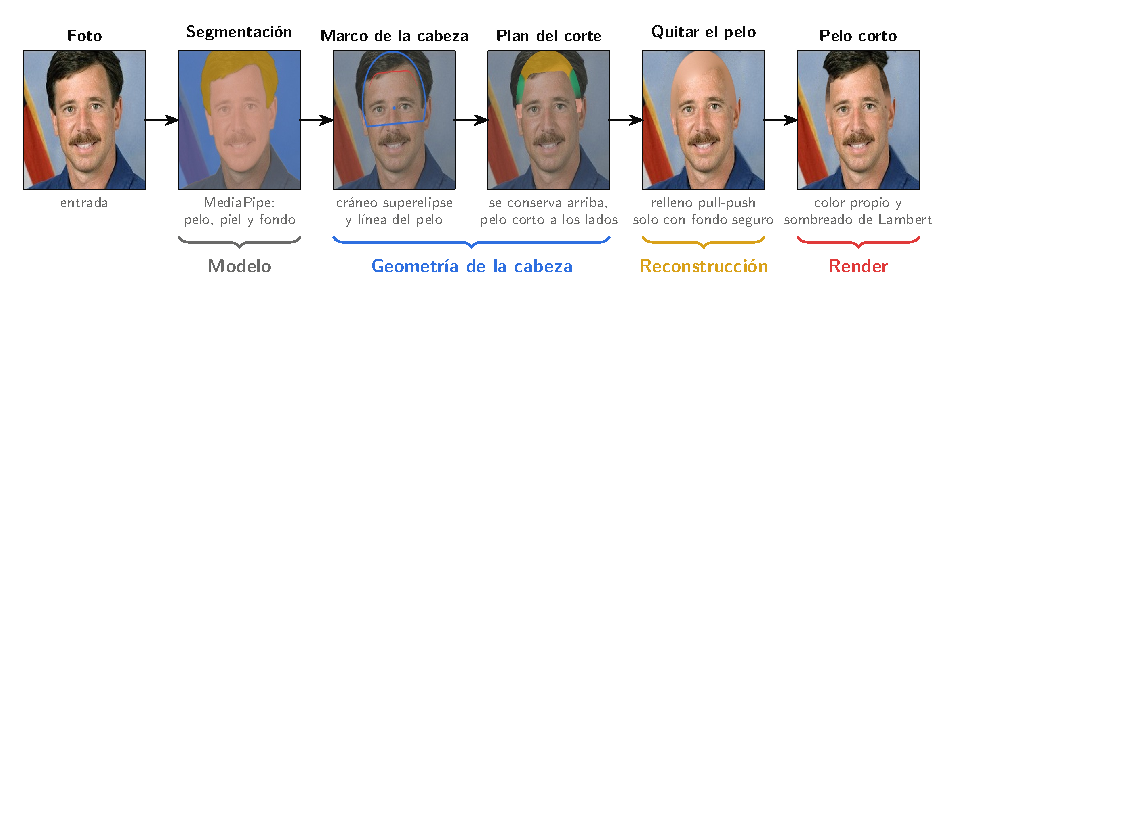
\includegraphics[width=0.95\textwidth]{diagrama_corte.pdf}
  \caption{Motor de cortes sobre un retrato de dominio público de la NASA (degradado medio): segmentación, marco de la cabeza con el cráneo y la línea del pelo, plan del corte, relleno con \emph{pull-push} y pelo corto sombreado.}
  \label{fig:corte}
\end{figure*}

\subsection{Motor de cortes}

Cortar el pelo exige quitarlo y reconstruir lo que había detrás (figura~\ref{fig:corte}). El \emph{inpainting} de Telea~\cite{telea2004} toma color de todo el borde del hueco, que incluye pelo, y deja ``pelo fantasma''. Usamos \emph{pull-push}~\cite{gortler1996}: una pirámide en la que solo cuentan como conocidos los píxeles de fondo seguro. El cráneo es una superelipse ajustada a la coronilla de cada persona,
\begin{equation}
  \left|\tfrac{x}{0{,}55}\right|^{2{,}15}+\left|\tfrac{\min(y,0)}{y_{\text{tope}}}\right|^{2{,}15}\le 1,
\end{equation}
y la línea del pelo sale de la frente visible o, con flequillo, de proporciones típicas~\cite{farkas1994}. El pelo corto toma el color propio y se sombrea con Lambert~\cite{marschner2016}, con la luz estimada de la asimetría de brillo de la cara. Los ocho cortes son tablas de parámetros sobre el mismo marco.

\subsection{Física de la barba y juego}

En el modo en vivo, cada hebra es una cadena de cuatro partículas con la raíz anclada a la piel por coordenadas baricéntricas. Se integra con Verlet~\cite{verlet1967} amortiguado, $x\leftarrow x+0{,}86\,(x-x_{\text{prev}})+g\,h^2$, y restricciones de distancia (PBD)~\cite{jakobsen2001,muller2007} que mantienen el largo. Cada tramo se dibuja como una gaussiana 2D y se acumula con $\alpha=1-e^{-A}$. En el juego Contrarreloj, el dedo índice corta las hebras cercanas al segmento recorrido entre dos cuadros (una cápsula), porque a 10 cuadros por segundo el dedo salta.

\subsection{Gaussianas 2D y 3D}

Un retrato se reconstruye como suma de $N$ gaussianas 2D, al estilo de GaussianImage~\cite{zhang2024}. Cada una guarda el factor de Cholesky de la inversa de su covarianza, $\Sigma^{-1}=LL^\top$, para que siempre sea válida, y se optimiza con gradientes analíticos y Adam~\cite{kingma2015} escritos a mano, sin PyTorch.

El espejo 3D construye, desde una foto y la malla 3D de MediaPipe, más de 100\,000 gaussianas en forma de discos tangentes, y las dibuja con un visor propio en WebGL2. El \emph{vertex shader} proyecta cada covarianza con EWA~\cite{zwicker2001},
\begin{equation}
  \Sigma_{2D}=J\,W\,\Sigma\,W^\top J^\top+0{,}3\,I,
\end{equation}
un \emph{counting sort} las ordena de atrás hacia adelante y el \emph{fragment shader} las mezcla, como en 3D Gaussian Splatting~\cite{kerbl2023}. La peluca 3D, en cambio, escanea el peinado con la cámara y obtiene su forma con una envolvente visual~\cite{laurentini1994} calculada rebanada por rebanada.

\section{Resultados}

La figura~\ref{fig:cortes} muestra los ocho cortes sobre tres personas con pelo distinto: en todos el fondo queda limpio y la cara no cambia. La tabla~\ref{tab:resultados} reúne las cifras principales. Además de los retratos de la NASA, los cortes y el tinte se revisaron sobre 26 caras distintas, y 54 pruebas automáticas corren en GitHub Actions en cada cambio.

\begin{figure*}[t]
  \centering
  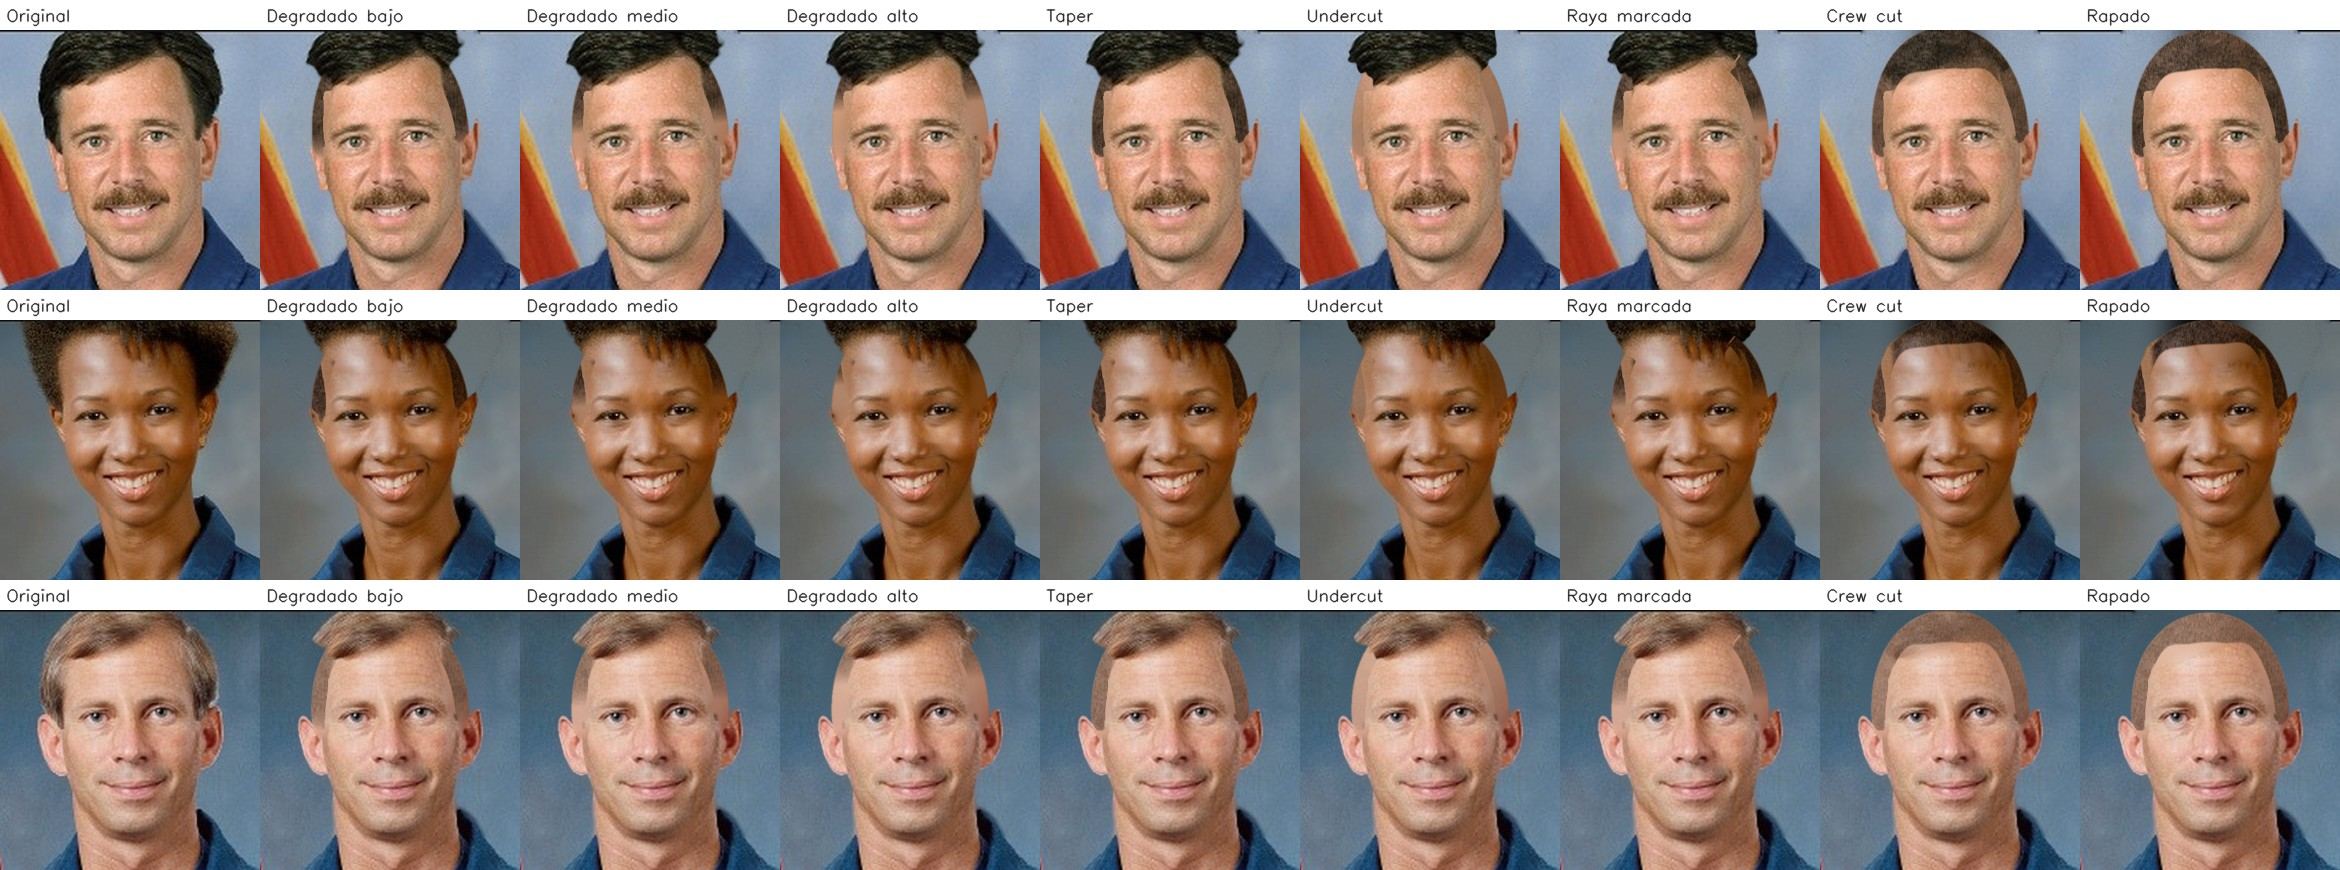
\includegraphics[width=\textwidth]{cortes.jpg}
  \caption{Los ocho cortes sobre tres retratos de dominio público: degradado bajo, medio y alto, \emph{taper}, \emph{undercut}, raya marcada, \emph{crew cut} y rapado.}
  \label{fig:cortes}
\end{figure*}

\begin{table}[t]
\centering
\small
\begin{tabular}{@{}lr@{}}
\toprule
Medida & Valor \\
\midrule
Corte, foto de 1024--1638~px (CPU) & 0,6 -- 1,9~s \\
Corte, foto de 4000~px & 0,8 -- 1,1~s \\
Tinte con YOLO y barba & 2,5~s \\
Espejo 3D (105\,000 gaussianas) & 2,6~s \\
Barba en vivo, por cuadro & 61~ms \\
Física en vivo, por cuadro & 72~ms \\
\midrule
YOLO de pelo: mAP50 de máscara & 0,968 \\
IoU entre YOLO y MediaPipe & 0,82 -- 0,94 \\
Gaussianas 2D: PSNR con 20 y 2000 & 18,4 y 34,5~dB \\
Delaunay con 83 puntos & 3~ms \\
\bottomrule
\end{tabular}
\caption{Tiempos y calidad. El PSNR sube unos 8~dB cada vez que se multiplica por 10 el número de gaussianas.}
\label{tab:resultados}
\end{table}

\section{Limitaciones}

\begin{itemize}
  \item Si una mano pasa delante de la cara en vivo, la barba se dibuja encima.
  \item Si un flequillo largo tapa un ojo, el rapado deja mechones, porque nunca se modifica la cara.
  \item El espejo 3D usa una sola vista: no tiene nuca y el relieve se estira con giros grandes.
  \item El modo en vivo corre a unos 10 cuadros por segundo, porque cada cuadro se procesa en el servidor.
\end{itemize}

\section{Conclusiones}

Fresh muestra que se puede probar un estilo de barbería de forma creíble sin modelos generativos: basta con ubicar la cara y el pelo, y resolver el resto con geometría, color, relleno de imágenes, física y \emph{splatting}. Cada pieza es explicable y corre en CPU. Como trabajo futuro quedan el tinte en vivo con un \emph{shader} de WebGL y un 3D Gaussian Splatting entrenado con varias vistas para completar la cabeza.

\paragraph{Aportes.} Kalos Lazo: arquitectura, tinte, YOLO, motor de cortes, forma de cara, interfaz y despliegue. Gianpier Segovia: barba, Delaunay de Fortune, \emph{warp}, física, gaussianas 2D, juego y espejo 3D. Sofía Herrera: peluca 3D y laboratorio.

\paragraph{Disponibilidad.} El código, el informe completo con todas las fórmulas y la guía de uso están en el repositorio del proyecto. La aplicación se levanta con \texttt{docker compose up -d --build app}.

{\small
\bibliographystyle{ieeetr}
\bibliography{references}
}

\end{document}
